\documentclass{beamer}

\mode<presentation>
{
   \usetheme{EEng}
%   \usetheme{Warsaw}
  \setbeamercovered{transparent}
  \setbeamercolor{background canvas}{bg=black!0}
}

\usepackage{enumerate}
\usepackage{array}
\usepackage{graphics}
\usepackage{ucs}
\usepackage[utf8x]{inputenc}
\usepackage[english]{babel}
\usepackage{amsmath, amsthm, amssymb}
\usepackage{amsmath}
\usepackage{amsfonts}
\usepackage{xcolor}
\usepackage{pgf}
\usepackage{hyperref}
\usepackage{url}
\usepackage{multicol}   % add-on
\usepackage{boxedminipage} 
\usepackage{indentfirst}   % add-on
\usepackage{float}
\usepackage{listings}
\usepackage{verbatim}
\usepackage{boxedminipage}

% % % inicio do listings e ref
\definecolor{darkblue}{rgb}{0,0,0.6}
\definecolor{gray_ulisses}{gray}{0.55}
\definecolor{castanho_ulisses}{rgb}{0.71,0.33,0.14}
\definecolor{preto_ulisses}{rgb}{0.41,0.20,0.04}
\definecolor{green_ulises}{rgb}{0.2,0.75,0}

\hypersetup{
	a4paper,
	pdftex,
	bookmarks,
	colorlinks,
    citecolor=darkblue,
    linkcolor=darkblue,
    urlcolor=darkblue,
    filecolor=darkblue
}

\lstdefinelanguage{Terminall} {
       basicstyle=\scriptsize\ttfamily,
       breaklines=true,
       breakautoindent=false,
       showstringspaces=false
}
\lstdefinelanguage{Terminal} {
       basicstyle=\tiny\ttfamily,
       breaklines=true,
       breakautoindent=false,
       showstringspaces=false
}
\definecolor{gray_ulisses}{gray}{0.55}
\definecolor{castanho_ulisses}{rgb}{0.71,0.33,0.14}
\definecolor{preto_ulisses}{rgb}{0.41,0.20,0.04}
\definecolor{green_ulises}{rgb}{0.2,0.75,0}

\lstdefinelanguage{HaskellUlisses}
{
        basicstyle=\ttfamily\scriptsize,
        %backgroundcolor=\color{yellow},
        %frameshape={RYRYNYYYY}{yny}{yny}{RYRYNYYYY}, %contornos... muito nice...
        sensitive=true,
        morecomment=[l][\color{gray_ulisses}\ttfamily\tiny]{--},
        morecomment=[s][\color{gray_ulisses}\ttfamily\tiny]{\{-}{-\}},
        morestring=[b]",
        stringstyle=\color{red},
        showstringspaces=false,
%       numbers=left,
%       firstnumber=\thelstnumber,
        numberstyle=\tiny,
        numberblanklines=true,
        showspaces=false,
        breaklines=true,
        showtabs=false,
%       xleftmargin=15pt,
%       xrightmargin=-20pt,
        emph=
        {[1]
                FilePath,IOError,abs,acos,acosh,all,and,any,appendFile,approxRational,asTypeOf,asin,
                asinh,atan,atan2,atanh,basicIORun,break,catch,ceiling,chr,compare,concat,concatMap,
                const,cos,cosh,curry,cycle,decodeFloat,denominator,digitToInt,div,divMod,drop,
                dropWhile,either,elem,encodeFloat,enumFrom,enumFromThen,enumFromThenTo,enumFromTo,
                error,even,exp,exponent,fail,filter,flip,floatDigits,floatRadix,floatRange,floor,
                fmap,foldl,foldl1,foldr,foldr1,fromDouble,fromEnum,fromInt,fromInteger,fromIntegral,
                fromRational,fst,gcd,getChar,getContents,getLine,head,id,inRange,index,init,intToDigit,
                interact,ioError,isAlpha,isAlphaNum,isAscii,isControl,isDenormalized,isDigit,isHexDigit,
                isIEEE,isInfinite,isLower,isNaN,isNegativeZero,isOctDigit,isPrint,isSpace,isUpper,iterate,
                last,lcm,length,lex,lexDigits,lexLitChar,lines,log,logBase,lookup,map,mapM,mapM_,max,
                maxBound,maximum,maybe,min,minBound,minimum,mod,negate,not,notElem,null,numerator,odd,
                or,ord,otherwise,pi,pred,primExitWith,print,product,properFraction,putChar,putStr,putStrLn,quot,
                quotRem,range,rangeSize,read,readDec,readFile,readFloat,readHex,readIO,readInt,readList,readLitChar,
                readLn,readOct,readParen,readSigned,reads,readsPrec,realToFrac,recip,rem,repeat,replicate,return,
                reverse,round,scaleFloat,scanl,scanl1,scanr,scanr1,seq,sequence,sequence_,show,showChar,showInt,
                showList,showLitChar,showParen,showSigned,showString,shows,showsPrec,significand,signum,sin,
                sinh,snd,span,splitAt,sqrt,subtract,succ,sum,tail,take,takeWhile,tan,tanh,threadToIOResult,toEnum,
                toInt,toInteger,toLower,toRational,toUpper,truncate,uncurry,undefined,unlines,until,unwords,unzip,
                unzip3,userError,words,writeFile,zip,zip3,zipWith,zipWith3,listArray,doParse
        },
        emphstyle={[1]\color{blue}},
        emph=
        {[2]
                Bool,Char,Double,Either,Float,IO,Integer,Int,Maybe,Ordering,Rational,Ratio,ReadS,ShowS,String,
                Word8,InPacket
        },
        emphstyle={[2]\color{castanho_ulisses}},
        emph=
        {[3]
                case,class,data,deriving,do,else,if,import,in,infixl,infixr,instance,let,
                module,of,primitive,then,type,where
        },
        emphstyle={[3]\color{preto_ulisses}\textbf},
        emph=
        {[4]
                quot,rem,div,mod,elem,notElem,seq
        },
        emphstyle={[4]\color{castanho_ulisses}\textbf},
        emph=
        {[5]
                EQ,False,GT,Just,LT,Left,Nothing,Right,True,Show,Eq,Ord,Num
        },
        emphstyle={[5]\color{preto_ulisses}\textbf}
}
% % % fim do listings e ref

% % % inicio da definicao de comandos

% % % fim da definicao de comandos

\title{SAAP - Software para Análise e Avaliação de Programas}
\author{José Pedro Silva \and
Pedro Faria \and
Ulisses Costa
}

\date{\today}
\institute{Engenharia de Linguagens\\
Projecto integrado
}

\AtBeginSubsection[] {
  \begin{frame}<beamer>
    \frametitle{Index}
    \scriptsize{\tableofcontents[currentsection,currentsubsection]}
  \end{frame}
}

\AtBeginSection[] {
  \begin{frame}<beamer>
    \frametitle{Index}
    \scriptsize{\tableofcontents[currentsection]}
  \end{frame}
}
\begin{document}
\begin{frame}
   \titlepage
\end{frame}

\section{Motivação e Tecnologias}
\pgfdeclareimage[width=.8\textwidth]{topo}{images/topo}

\begin{frame} \frametitle{Motivação e Objectivos}
Aprofundar e demonstrar conhecimentos em:
\begin{itemize}
\item Desenhar arquitectura de um sistema de informação
\item Desenvolvimento web
\item Linguagens de Scripting
\item Bases de dados
\item Processamentos de texto
\end{itemize}
\end{frame}

\begin{frame} \frametitle{Tecnologia}
Principais ferramentas a usar:
\begin{itemize}
\item RoR - interface web
\item Perl - scripting
\item DB2 - motor de base de dados
\item Haskell
\end{itemize}
\end{frame}

\section{Contextualização}
\begin{frame} \frametitle{Descrição do Sistema}
Descrição do sistema e funcionalidades:
\begin{itemize}
\item Disponivel através de uma interface web
\item Criação de concursos e enunciados
\item Permite a submissão de programas
\item Avalia os programas submetidos
\item Gera métricas para programas existentes no sistema
\end{itemize}
\end{frame}

\begin{frame} \frametitle{Utilizadores do sistema - Docente}
\begin{itemize}
\item Pode criar, editar e eliminar concursos e enunciados
\item Pedir ao sistema para gerar métricas
\item Consultar todo o tipo de resultados
\end{itemize}
\end{frame}

\begin{frame} \frametitle{Utilizadores do sistema}
\begin{description}
\item[Admin] Entidade com mais poder no sistema, pode criar contas para docentes
\item[Grupo] Pode submeter ficheiros que serão avaliados pelo sistema
\end{description}
\end{frame}

\section{Modelação}
\begin{frame} \frametitle{Modelação informal da arquitectura}
\begin{figure}[htbp]
\begin{center}
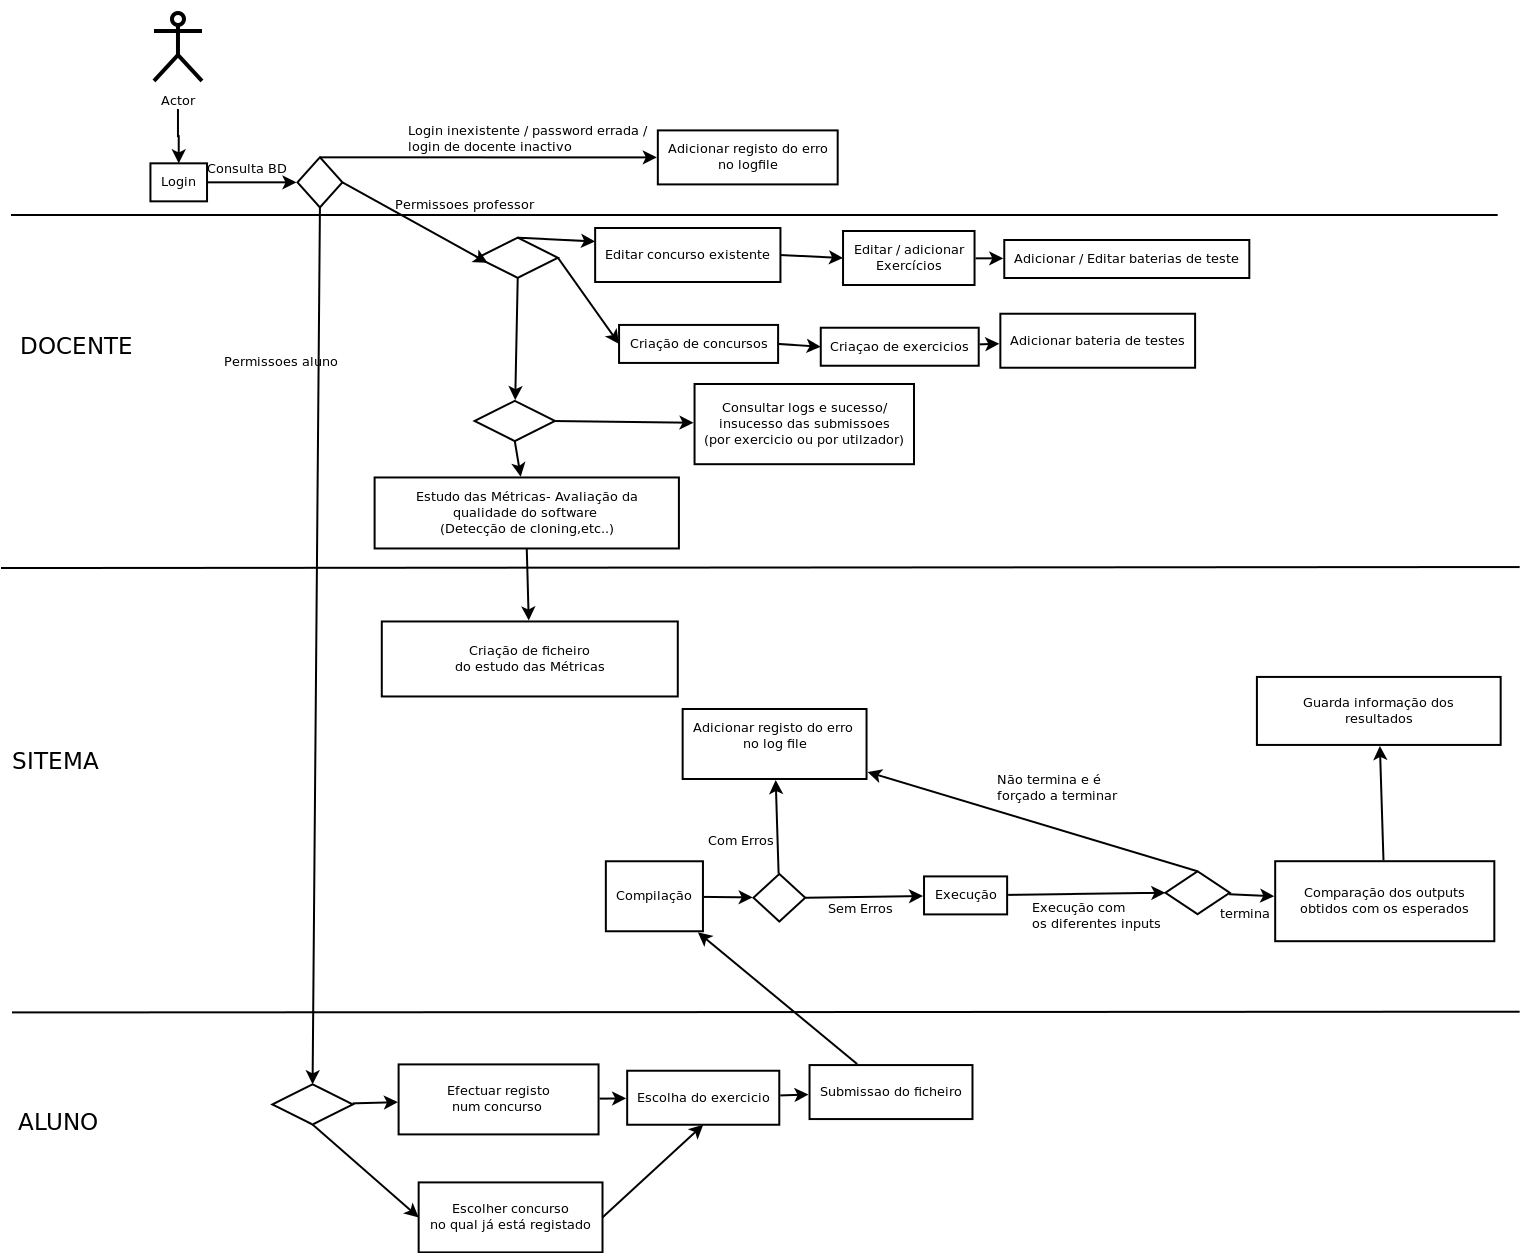
\includegraphics[width=0.8\textwidth]{../report1/Images/EL-PI}
\end{center}
\end{figure}
\end{frame}

\newcommand{\rarrow}{\rightarrow}
\newcommand{\larrow}{\leftarrow}
\newcommand{\unif}{\sim}
\def\prop#1#2#3{\noindent\\\begin{array}{l} \{#1\} \\ #2 \\ \{#3\} \\ \end{array}\\\\}

\begin{frame} \frametitle{Modelação formal}
\begin{displaymath}
\begin{array}{l}
\prop
{existsInDatabase(u)}
{login :: u \unif Username \times Hash \rarrow SessionID \rarrow Error + SessionID}
{ }
\end{array}
\end{displaymath}
\\
\begin{displaymath}
\begin{array}{l}
\prop
{ existeSession(s)  \wedge isProf(s) \wedge (notEmpty \circ getExercice)~c}
{createContest :: s \unif SessionID \rarrow c \unif Contest \rarrow 1}
{ (notEmpty \circ getDict)~c }
\end{array}
\end{displaymath}
\end{frame}

\begin{frame} \frametitle{Modelação formal}
$\begin{array}{l}
data~Dict~a~b = (a \times b)^{*} \\
data~Exercicio = Exercicio~Enunciado~(Dict~Input~Output) \\
data~Contest =  Contest~Nome~Tipo~Exercicio^{*}
\end{array}$\\
\begin{displaymath}
\begin{array}{l}
\prop
{ existeSession(s)  \wedge isProf(s) \wedge (not \circ exist) (Exercicio~e~d)}
{createExercice :: s\unif SessionID \rarrow e \unif Enunciado \rarrow d \unif (Dict~a~b) \rarrow 1}
{ exerciceCreated(Exercicio e d) }
\end{array}
\end{displaymath}
\end{frame}

\begin{frame} \frametitle{Modelação formal}
\begin{displaymath}
\begin{array}{l}
\prop
{ existSession(s) \wedge contestNotFull(c)}
{registerOnContest :: s \unif SessionID \rarrow c\unif Contest \rarrow Credenciais}
{ }
\end{array}
\end{displaymath}
\\
\begin{displaymath}
\begin{array}{l}
\prop 
{ existeSession(s) \wedge isProf(s) \wedge contestIsClosed(c) }
{consultarLogsContest :: s \unif SessionID \rarrow c \unif Contest \rarrow LogsContest}
{}
\end{array}
\end{displaymath}
\end{frame}

\begin{frame} \frametitle{Modelação formal}
\begin{displaymath}
\begin{array}{l}
\prop
{ }
{geraReport :: e \unif Exercicio \rarrow res \unif Resolucao \rarrow Report}
{ }
\end{array}
\end{displaymath}
\\
\begin{eqnarray*}
geraReportBugCompile :: Exercicio \rarrow Error \rarrow Report\\
geraReportBugCompare :: Exercicio \rarrow Errado \rarrow Report\\
geraReportNoBug :: Exercicio \rarrow Resolucao \rarrow Report\\
\\
execute :: Program \rarrow Exercicio \rarrow ResolucaoProposta\\
\end{eqnarray*}
\end{frame}

\begin{frame}[fragile] \frametitle{Modelação formal}
\begin{lstlisting}[language=HaskellUlisses]
geraReport :: Exercicio -> Resolucao -> Report
geraReport exer res = do
    case compile res of
    (Left error) -> geraReportBugCompile error res
    (Right p) ->
        let resProps = execute p exer
        in case (compare exer resProps) of
            (Left certo) -> geraReportNoBug e res
            (Right errado) -> geraReportBugCompare errado res
\end{lstlisting}

\begin{lstlisting}[language=HaskellUlisses]
geraReport exer res =
    compile res >>= \p -> compare exer (execute p exer)
        >>= \c -> geraReportNoBug exer res
\end{lstlisting}
\end{frame}

\subsection{Modelação de dados}

\begin{frame} \frametitle{Modelo de dados - Concurso, tentativa e enunciado}
\begin{figure}[htbp]
\begin{center}
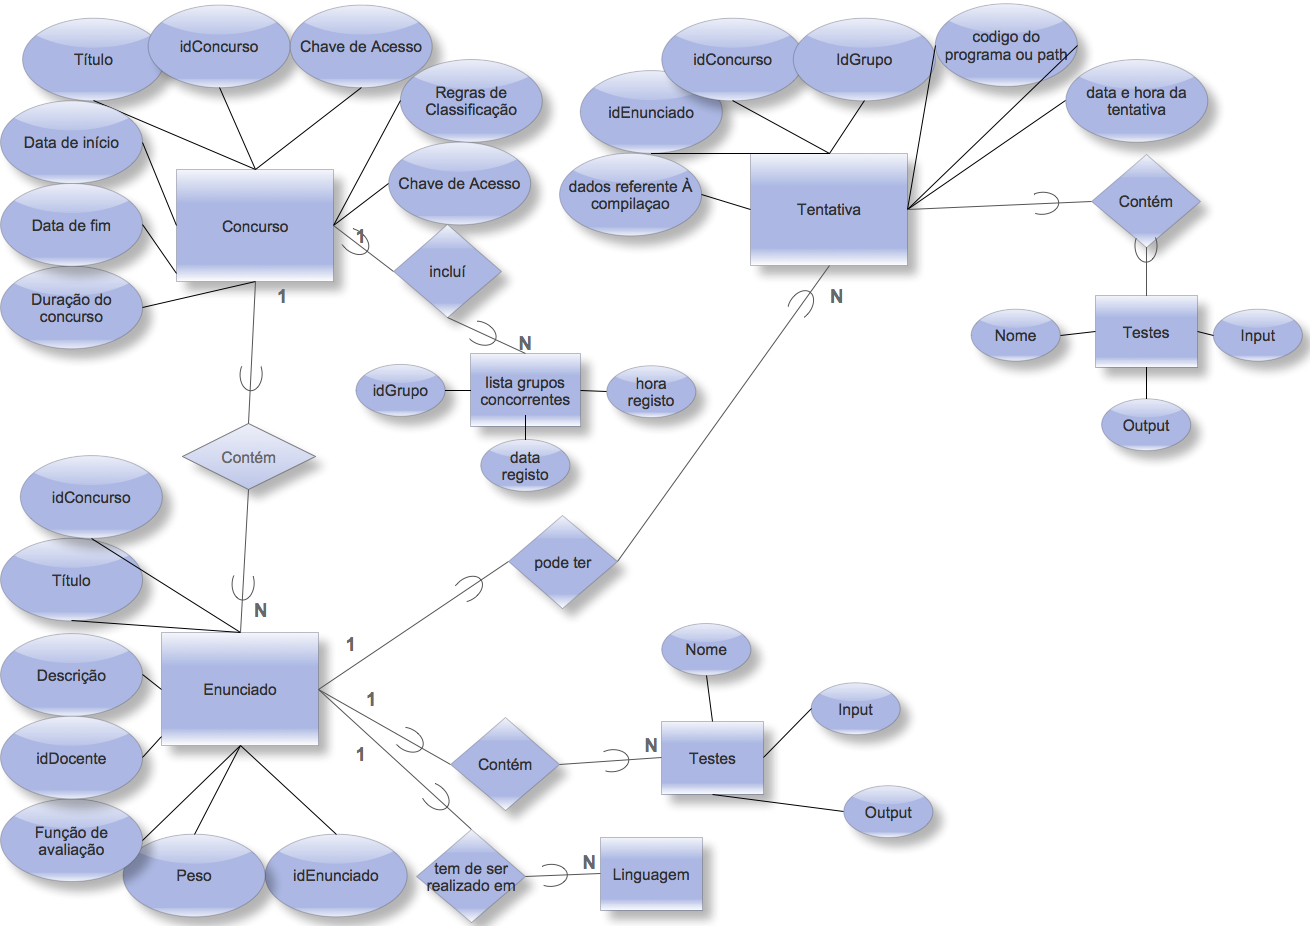
\includegraphics[width=0.9\textwidth]{../report1/Images/concurso-enunciado}
\end{center}
\end{figure}
\end{frame}


\begin{frame} \frametitle{Modelo de dados - Grupo e Doecente/Admin}
\begin{figure}[htbp]
\begin{center}
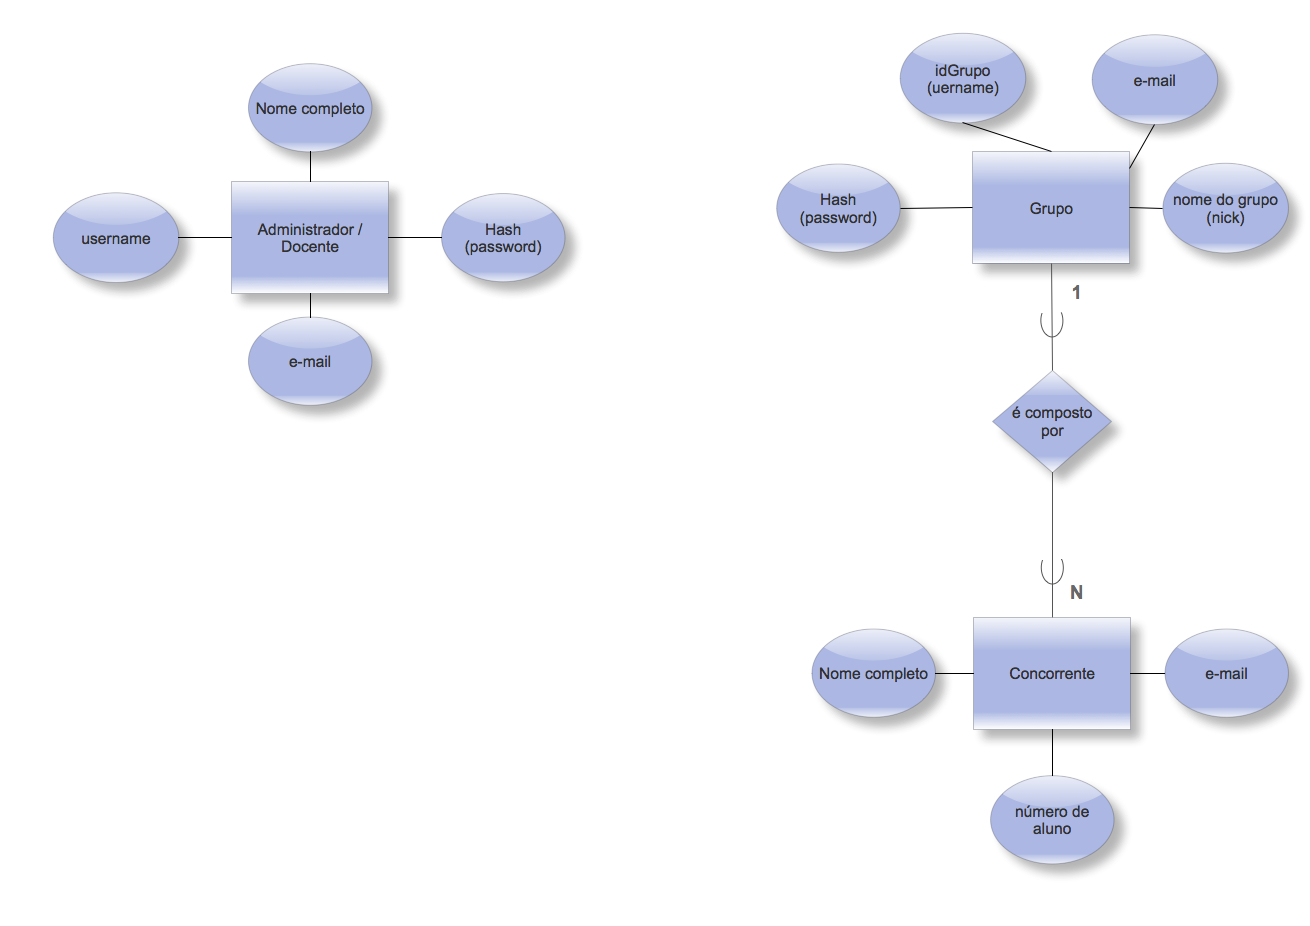
\includegraphics[width=0.9\textwidth]{../report1/Images/grupo-docente}
\end{center}
\end{figure}
\end{frame}

\subsubsection{XML}
\begin{frame}[fragile] \frametitle{Modelo de dados - XML - Enunciado}
\begin{lstlisting}[language=XML,basicstyle=\tiny,breaklines=true]
<?xm l version="1.0" encoding="UTF-8"?>
<Enunciado xmlns:xsi="http://www.w3.org/2001/XMLSchema-instance"
    xsi:noNamespaceSchemaLocation="enunciado.xsd">
    <idConcurso> 1 </idConcurso>
    <Peso>20</Peso>
    <Titulo> Exercicio 1 </Titulo>
    <Descricao> Some os numeros que lhe sao passados como argumento, e apresente o resultado. </Descricao>
    <Exemplo>Input: 1 1 1 1 1   Output: 5</Exemplo>
    <Docente> PRH </Docente>
    <FuncAval>Diff</FuncAval>  
    <Linguagens> 
        <Linguagem>C</Linguagem>        
    </Linguagens> 
\end{lstlisting}
\end{frame}

\begin{frame}[fragile] \frametitle{Modelo de dados - XML - Enunciado - Part2}
\begin{lstlisting}[language=XML,basicstyle=\tiny,breaklines=true]
    <Dict>
        <Teste>
            <Nome>Lista vazia</Nome>
            <Input></Input>
            <Output>0</Output>
        </Teste>
        <Teste>
            <Nome>Lista c/ 1 elem</Nome>
            <Input>1</Input>
            <Output>1</Output>
        </Teste>
        <Teste>
            <Nome>Lista c/ varios elem</Nome>
            <Input> 2 3 4 5 </Input>
            <Output>14</Output>
        </Teste>
    </Dict>
</Enunciado>
\end{lstlisting}
\end{frame}

\begin{frame}[fragile] \frametitle{Modelo de dados - XML - Tentativa}
\begin{lstlisting}[language=XML,basicstyle=\tiny,breaklines=true]
<?xm l version="1.0" encoding="UTF-8"?>
<Enunciado xmlns:xsi="http://www.w3.org/2001/XMLSchema-instance"
    xsi:noNamespaceSchemaLocation="tentativa.xsd">
    <idConcurso>1</idConcurso>
    <idEnunciado>1</idEnunciado>
    <idGrupo>36</idGrupo>
    
    <data>2010-12-08</data>
    <hora>16:33:00</hora>
    
    <compilou>1</compilou>
\end{lstlisting}
\end{frame}

\begin{frame}[fragile] \frametitle{Modelo de dados - XML - Tentativa - Part2}
\begin{lstlisting}[language=XML,basicstyle=\tiny,breaklines=true]
    <Dict>
        <Teste>
            <Nome>Lista vazia</Nome>
            <Input></Input>
            <Output>0</Output>
        </Teste>
        <Teste>
            <Nome>Lista c/ 1 elem</Nome>
            <Input>1</Input>
            <Output>1</Output>
        </Teste>
        <Teste>
            <Nome>Lista c/ varios elem</Nome>
            <Input> 2 3 4 5 </Input>
            <Output>14</Output>
        </Teste>
    </Dict>
    <pathMetricas>sasas</pathMetricas>
\end{lstlisting}
\end{frame}

\begin{frame}[fragile] \frametitle{Modelo de dados - XML - Tentativa - Part3}
\begin{lstlisting}[language=XML,basicstyle=\tiny,breaklines=true]
    <codigoFonte>
        <nome>prog.c</nome>
        <codigo>
            <![CDATA[
            #include <stdio.h>
            
            ...restante codigo...
            
            ]]>
        </codigo>
    </codigoFonte>
        
</Enunciado>
\end{lstlisting}
\end{frame}

\subsubsection{XSD}
\begin{frame}[fragile] \frametitle{Modelo de dados - excerto do XSD do Enunciado}
Exemplo de elemento com restrições:\\
\begin{lstlisting}[language=XML,basicstyle=\tiny,breaklines=true]
<ed:element name="Peso" default="25">
  <ed:simpleType>
    <ed:restriction base="ed:integer">
      <ed:minInclusive value="0"/>
      <ed:maxInclusive value="100"/>
    </ed:restriction>
  </ed:simpleType>
</ed:element>
\end{lstlisting}
\end{frame}

\begin{frame}[fragile] \frametitle{Modelo de dados - excerto do XSD do Enunciado}
Exemplo de elemento com restrições:\\
\begin{lstlisting}[language=XML,basicstyle=\tiny,breaklines=true]
<ed:element name="Linguagem" maxOccurs="unbounded">
    <ed:simpleType>
    <ed:restriction base="ed:string">
        <ed:enumeration value="C"/>
        <ed:enumeration value="Java"/>
        <ed:enumeration value="Haskell"/>
    </ed:restriction>
    </ed:simpleType>
</ed:element>
\end{lstlisting}
\end{frame}

\begin{frame}[fragile] \frametitle{Modelo de dados - Diagrama correspondete ao XSD do Enunciado}
\begin{figure}[htbp]
\begin{center}
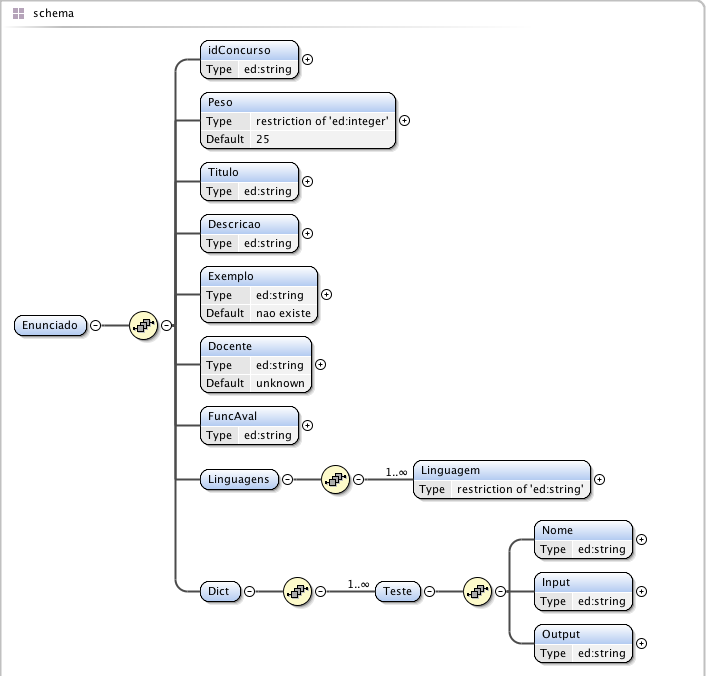
\includegraphics[width=0.7\textwidth]{../report1/Images/enunciado_schema}
\caption{diagrama do schema para o enunciado}\label{fig xsd enunciado}
\end{center}
\end{figure}
\end{frame}


\begin{frame}[fragile] \frametitle{Modelo de dados - excerto do XSD da Tentativa}
Exemplo de elemento que pode ocorrer mais do que uma vez:\\
\begin{lstlisting}[language=XML,basicstyle=\tiny,breaklines=true]
<tt:element name="Dict">
    <tt:complexType>
    <tt:sequence>
        <tt:element name="Teste" maxOccurs="unbounded">
        <tt:complexType>
            <tt:sequence>
            <tt:element name="Nome" type="tt:string"/>
            <tt:element name="Input" type="tt:string"/>
            <tt:element name="Output" type="tt:string"/>
            </tt:sequence>
        </tt:complexType>
        </tt:element>
    </tt:sequence>
    </tt:complexType>
</tt:element>
\end{lstlisting}
\end{frame}

\begin{frame}[fragile] \frametitle{Modelo de dados - Diagrama correspondete ao XSD da Tentativa}
\begin{figure}[htbp]
\begin{center}
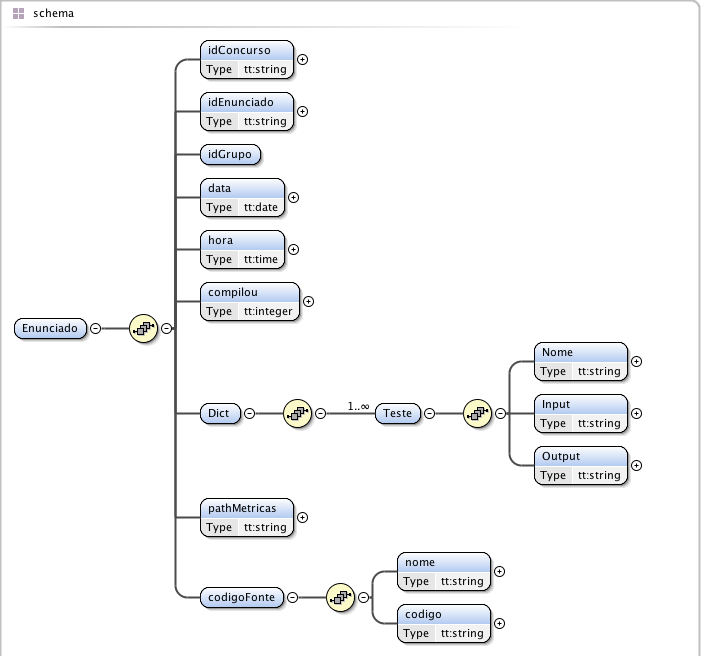
\includegraphics[width=0.7\textwidth]{../report1/Images/tentativa_schema}
\caption{diagrama do schema para a tentativa}\label{fig xsd tentativa}
\end{center}
\end{figure}
\end{frame}

\section*{Perguntas}
\begin{frame} \frametitle{Perguntas}
\begin{center}\huge{?}\end{center}
\end{frame}

\end{document}
